\section{Design and Theory}

A velocity field is a function taking as input a state, $q$ and returns a 3 dimensional desired velocity vector $(u,v,w)$.\\ It describes a path (a function of position) as opposed to a trajectory (function of position and time).

\subsection{Spherical field to maintain desired force }
When contact has been made, we suppose that the surface static friction coefficient is high enough to maintain the contact.
Since the arm has a fixed size and does not move, this section will describe a velocity field on the surface of a sphere around the target point with a radius defined by the distance between the CoM of the quadcopter and the tip of the arm.\\
Computing the field on the surface of a sphere is very computationally efficient because we do not have to sample field vectors in the whole 3d space around the point of interest.
First we need to compute the feasible position of the CoM to apply the desired force. 
We know that this position is unique because there is only one vertically stable pitch for a given desired force amplitude. The quadcopter needs to pitch to have a forward velocity because the quadcopter is underactuacted.\\
We can either compute this position analytically or we can use machine learning techniques such as regression to compute the feasible pitch as a function of the desired force. The latter option would require collecting training data from simulations on Gazebo. 
Now we can generate the velocity field on the surface of the sphere to point on the tangent direction of the sphere in the direction of the stable pitch position. \\
This field will have an amplitude proportional to the distance from this point.
The planning strategy we described would also allow us to easily define a desirable range for the yaw angle depending on the type of sensor and on the friction coefficient of the target surface.
Finally, we use a Passive Velocity Field Controller \cite{li1999passive} to follow this field to minimize the loss of kinetic energy to the environment when interacting with the surface.
Now we are going to describe how the spherical field is computed. 
Let us recall that the cartesian to spherical change of variable is defined as
\begin{equation} 
    r = \sqrt{x^2+y^2+z^2}\\ \nonumber 
\end{equation}
\begin{equation}
    \theta = \arccos(\frac{z}{r})\\\nonumber 
\end{equation}
\begin{equation}
    \label{transformation}
    \phi =
    \begin{cases}
        \arctan(\frac{y}{x}), & \text{if $x>0$},\\
        \arctan(\frac{y}{x}) + \pi, & \text{if $x<0$ and $y\geq 0$},\\
        \arctan(\frac{y}{x}) - \pi, & \text{if $x<0$ and $y<0$},\\
        \pi/2, & \text{if $x=0$ and $y>0$},\\
        -\pi/2, & \text{if $x=0$ and $y<0$},\\
        not defined , & \text{if $x=0$ and $y=0$}
    \end{cases}       
\end{equation}  
The jacobian defining the curvature of the sphere for at each point for this transformation is 
\begin{align}
    J = \frac{\partial{(x,y,z)}}{\partial{(r,\phi,\theta)}} \nonumber\\
    J = \begin{bmatrix}
        \sin(\theta)\cos(\phi) & \cos(\theta)\cos(\phi) & -\sin(\phi)\\
        \sin(\theta)\sin(\phi) & \cos(\theta)\sin(\phi) & \cos(\phi)\\
        \cos(\theta) & -\sin(\theta) & 0\\
        \end{bmatrix}
        \label{jacobian}
\end{align}

Figure \ref{fig:spherical} represents an example of such a field where the red point is the optimal position to apply the pressure, the blue arrows are the velocity field vectors and the center of the sphere is the point where the force is applied

\begin{figure*}[h!]
    \centering
    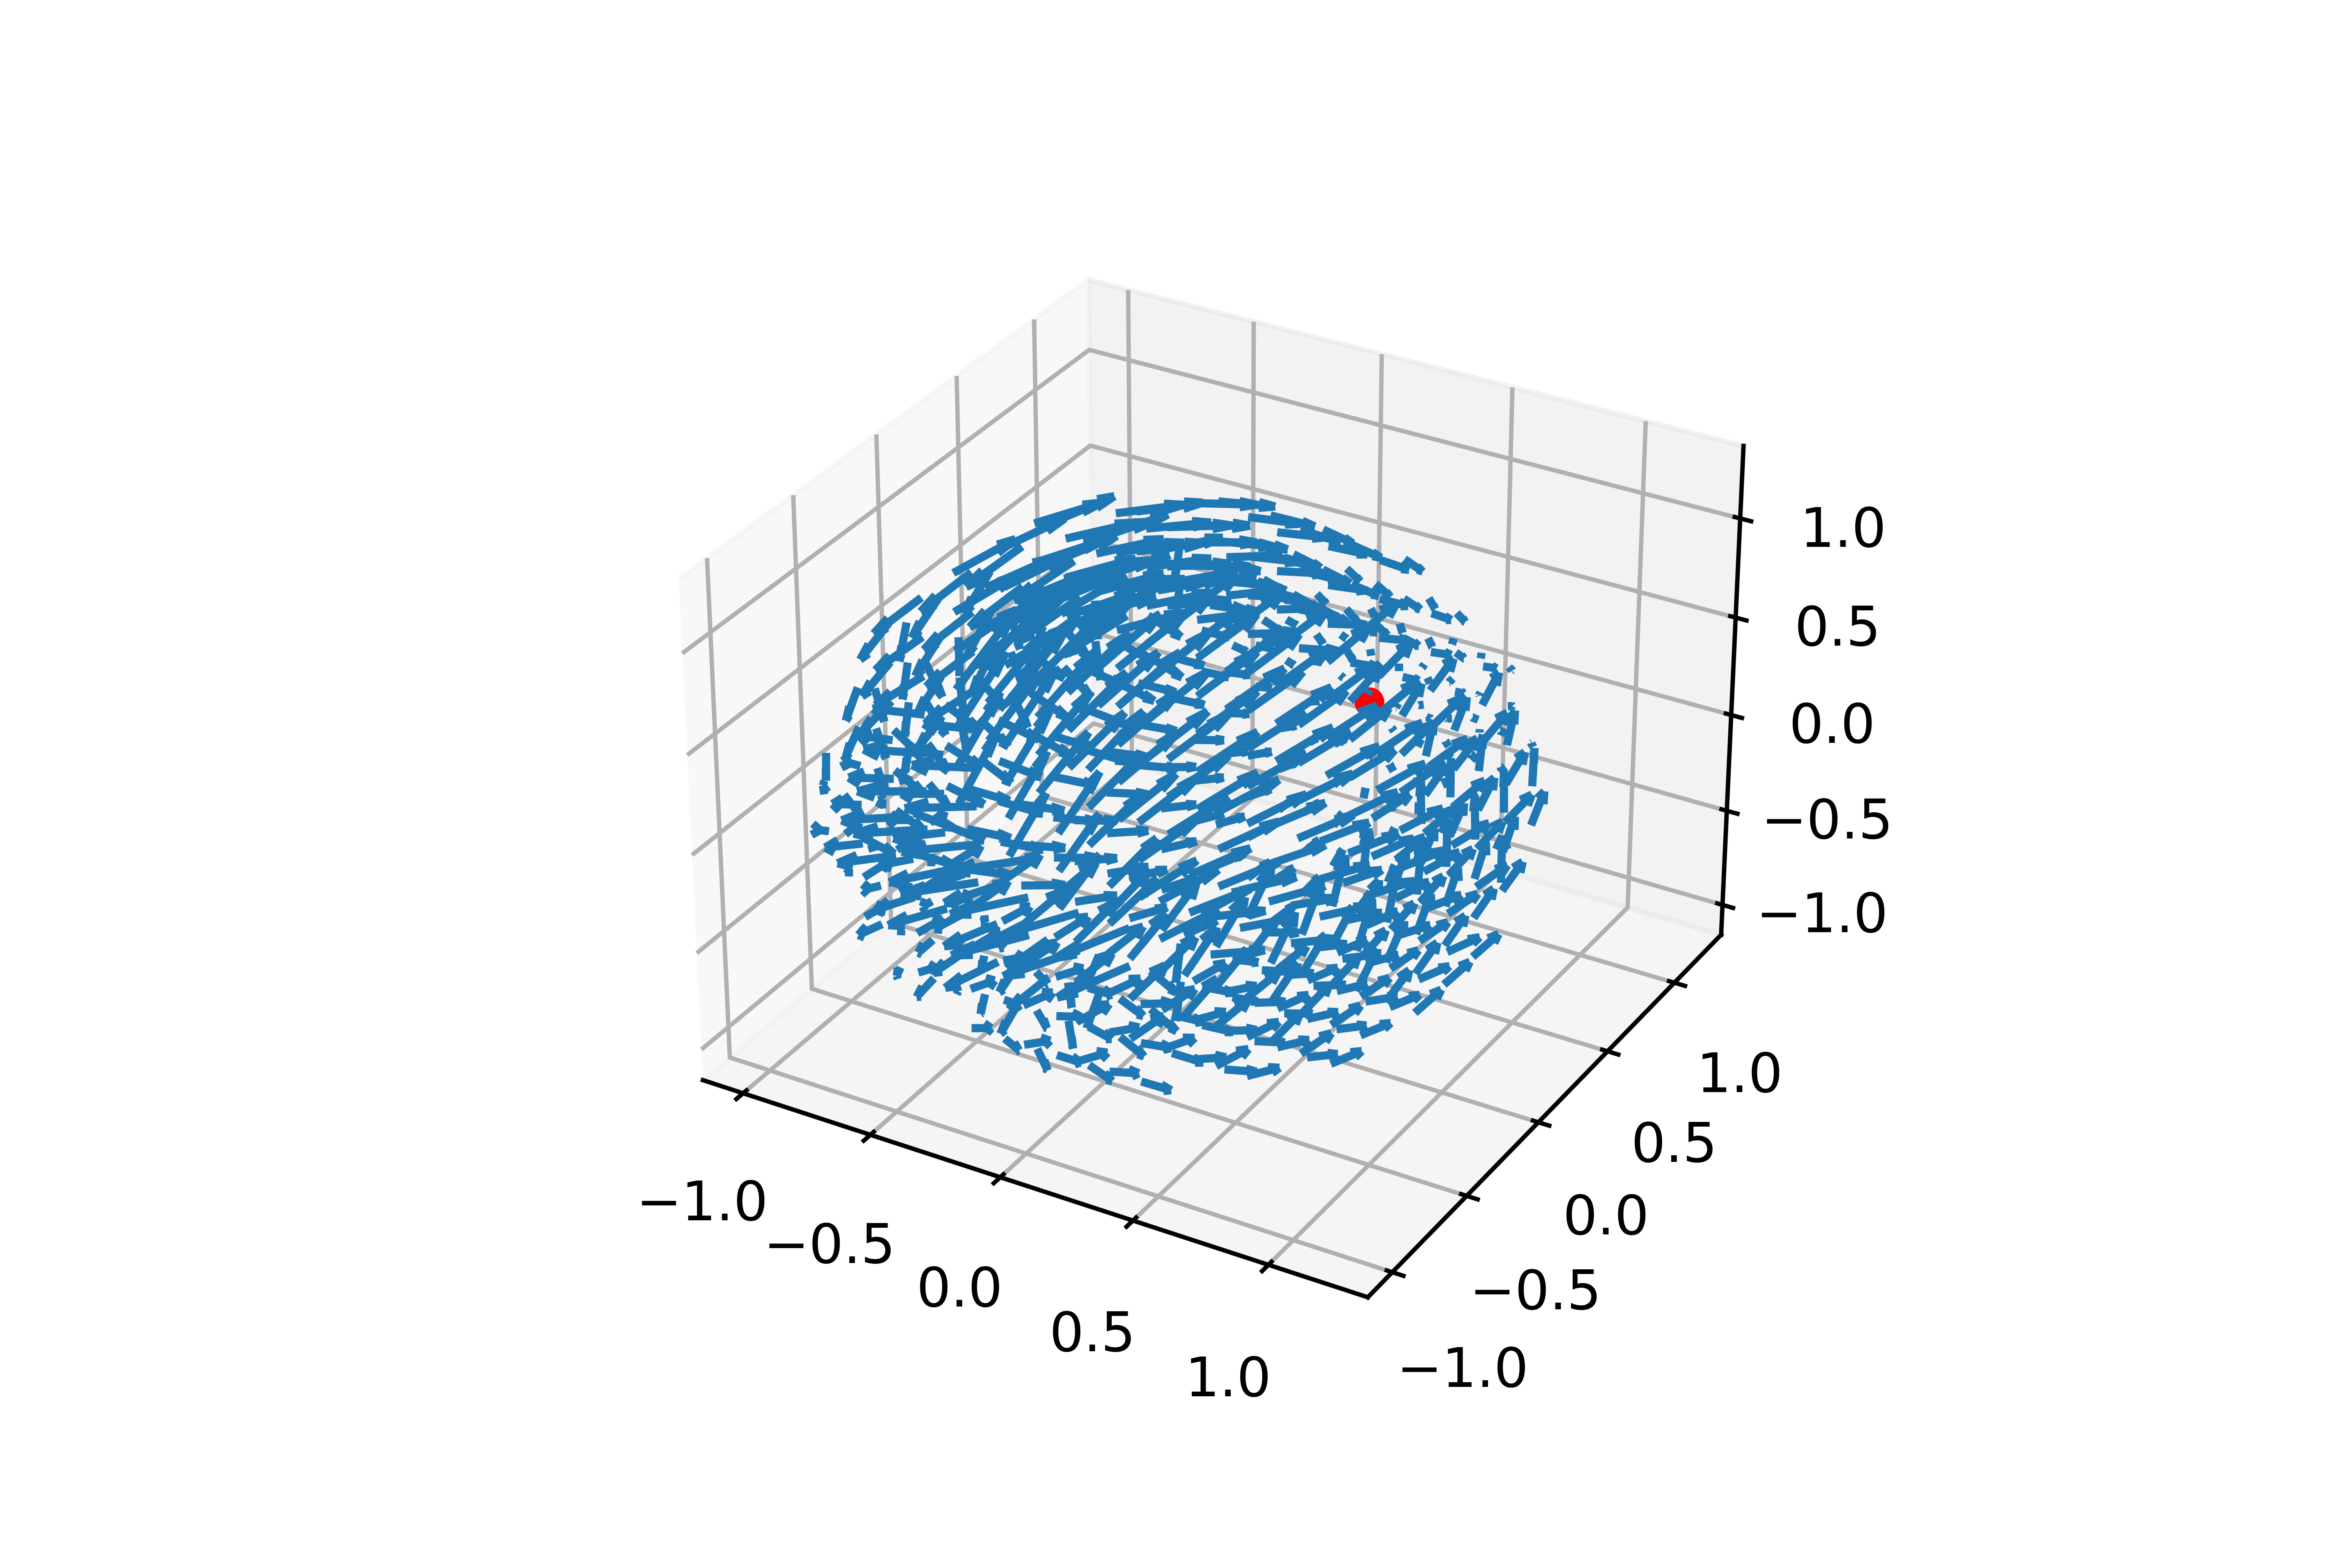
\includegraphics[width=\linewidth]{Images/sphericalfield.png}
    \caption{Spherical contact field}
    \label{fig:spherical}
\end{figure*}


\subsection{Passive Velocity Field Control of Mechanical Manipulators}
In \cite{li1999passive}, the author explains the advantages of encoding a contour following task using velocity fields. 
He later presents the passive velocity field controller whose objective is to "maintain an energetically passive relation-ship between the manipulator under closed loop control and
its physical environment, while causing the manipulator to perform the desired task." 
We will explain each one of those arguments and relate them to our sensor placement task.
\subsubsection{Velocity fields for planning}
The classical approach to do planning is to encode the task into a timed trajectory $Q:\mathbb R_{\ge 0} \rightarrow G$ where G is the n-dimensional configuration manifold for the manipulator and use a controller to minimize the state trajectory error.
Using this strategy, the objective of the controller is to minimize the deviation between $q(t)$ and $Q(t)$ where $q:\mathbb R_{\ge 0} \rightarrow G$ is the actual coordinate representation of the manipulator.
This strategy could be fine if the manipulator was able to never deviate from the timed trajectory defined by Q. However, if deviation occurs for example, when external forces are appllied to the
robot, a side effect of this minimization strategy called radial reduction can occur.

\begin{figure}[h!]
    \centering
    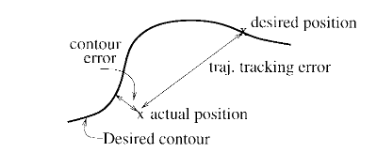
\includegraphics[width=0.48\textwidth]{Images/radialreduction.png}
    \caption{radial reduction from \cite{li1999passive}}
    \label{fig:radialreduction}
\end{figure} 
The author argues that if following the path of the desired trajectory is more important than the timing in which the manipulator follows this trajectory, a strategy based on velocity field is more appropriate because the velocity of the manipulator will only depend on its current position and will be time invariant.  
For the sensor placement task, using a timed trajectory strategy with deviation minimization to reach the contact point may lead the UAV to collide with an obstacle. With our strategy based on potential velocity field, the UAV will not try to shortcut the desired path in case of deviation.
The author defines an $\alpha$ error such that:
\begin{equation}
    e_{\alpha} = \dot{q} - \alpha V
\end{equation}
One of the most important priorities of PVFC is that when no external forces are applied on the robot, there is a positive $\alpha$ such that 
\begin{equation}
    \lim_{t\to\infty}e_{\alpha} = 0
\end{equation}
In other words, PVFC does not seek to exactly match the desired velocity field magnitude but just an $alpha$ scaled version of it. The $\alpha$ we are going to converge to is a function of the energy in the augmented system and the energy in the desired velocity field.
\subsubsection{Passive velocity field controller}
The controller presented in this paper allows storing kinetic energy of the manipulator's actuators in a spring or a flywheel and releasing it when needed so that we can interact with surfaces while minimizing energy loss. This is useful because the UAV has a limited amount of energy stored in its battery and this is one of the main limiting factors for most tasks (including Sensor Placement). \\
To present this concept, the author first define the notion of a passive dynamic system:\\
A dynamic system with input $u \in U$ and output $y \in Y$ is passive with respect to the supply rate 
$s:U \cross Y \rightarrow \mathbb R$, if for any $u: \mathbb R_{\ge 0} \rightarrow U $ and for any $t\geq 0$ the following relation is satisfied:
\begin{align}
    \exists ~ c\in\mathbb R  \nonumber\\
    \int_{0}^{t}s(u(\tau),y(\tau))d\tau \geq -c^2 \label{passivityCondition}
\end{align}

Let us remember that the work $W$ and power $P$ of a force $F$ on a point mass object with velocity $v$ are defined as
\begin{align}
    P = F.v\\
    W = \int_{0}^{t}P dt
\end{align}

Therefore the supply rate  $s(\tau_{tot},\dot{q})=\tau_{tot}^{T}\dot{q}$ can be seen as the total mechanical power input. Here the input $\tau_{tot}$ is the total force exerted on the manipulator 
and the output $\dot{q}$ is the velocity of the manipulator. 

When considering a feedback system interacting with the environement shown in figure \ref{fig:pvfccontrolloop}, we can decompose $\tau_{tot}=\tau_{e}+\tau$ (where $\tau$ and $\tau_{e}$ are respectively the forces generated by the actuators and the external forces, for example the contact force when touching a surface),
we can derive the power generated by external forces as $s(\tau_{e}\dot{q})=\tau_{e}^T \dot{q}$. 
\begin{figure}[h!]
    \centering
    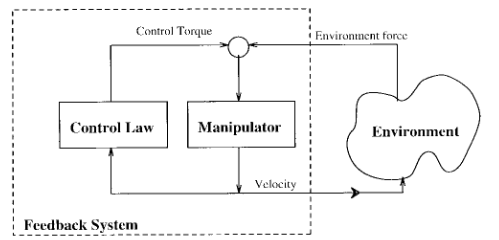
\includegraphics[width=0.48\textwidth]{Images/pvfccontrolloop.png}
    \caption{PVFC loop \cite{li1999passive}}
    \label{fig:pvfccontrolloop}
\end{figure} 
As explained in the paper, a system defined by this supply rate is not passive because obstacles may bring the manipulator to a complete stop for an unbounded amount of time and this loss of kinetic enery cannot be bounded. 
As a result, the passivity relation 
\begin{equation}
    \int_{0}^{t}\tau_{e}^T \dot{q}d\tau \geq -c^2 
\end{equation}
is not valid here because the l.h.s represents the total amount of energy lost to the environment and, as stated before, it cannot be bounded. 
This issue motivates the introduction of an augmented system: a fictitious flywheel is added to the system that acts as an energy storage element.
The dimensionality of the manifold is then increased by one to include the state of the flywheel and this augmented state will be noted as
\begin{align} 
    \bar{q}=[q_1,...,q_n,q_{n+1}]
    \bar{V} = [V, V_fly]
\end{align}

\subsubsection{Augmented dynamics}
Let us now describe the dynamics of the augmented system
\begin{equation} 
    \bar{M}(\bar{q})\ddot{\bar{q}} + \bar{C}(\bar{q}, \dot{\bar{q}})\dot{\bar{q}} = \bar{\tau} + \bar{\tau_{e}}
\end{equation}
The mass matrix of the augmented system is defined such that:
\begin{align}
\bar{M}(q) = \begin{bmatrix} 
   M(q) & 0 \\
    0 & m_f
\end{bmatrix}\\
M(q) =  \begin{bmatrix} 
    m_b & 0 & 0 \\
    0 & m_b & 0 \\
    0 & 0 & m_b \\
 \end{bmatrix}
\end{align}
The Coriolis Matrix of the augmented system is defined such that: 
\begin{align}
\bar{C}(\bar{q}, \dot{\bar{q}}) = \begin{bmatrix} 
    C(q, \dot(q)) & 0 \\
    0 & 0 
\end{bmatrix}
\end{align}
$C$ is built using the Levi–Civita connection describe in pvfc part1
\subsubsection{Augmented velocity field}
Now let us define the augmented field for the flywheel. The motivation for introducing an augmented system is
to allow energy transfer between the quadcopter actuators and the flywheel such that the total kinetic energy in the system remains constant.
This property is enforced in the definition of the desired velocity field. \\
First let us define $\bar{E}$ to be the total energy of the augmented system following the desired velocity field.
$\bar{E}$ can be written as a sum of the flywheel desired kinetic energy $K_{fly_{d}}$ and the quad desired kinetic energy $K_{quad_{d}}$: 
\begin{equation}
    \bar{E} = K_{fly_{d}} + K_{quad_{d}}
\end{equation}
Given a desired velocity field $V$ we have: 
\begin{equation}
    K_{quad_{d}}(q) = V(q)^T\frac{1}{2}M(q)V(q)
\end{equation}
Since 
\begin{equation}
    K_{fly_{d}} = \frac{1}{2} m_f V_fly
\end{equation}
We can derive $V_fly$ in function of  $K_{quad_{d}}(q)$ and $E_bar$:
\begin{equation}
    V_{fly}(q) = \sqrt(\frac{2}{m_f}(\bar{E}- K_{quad_{d}}(q)))
\end{equation}
\subsubsection{PVFC Control law}
To define the PVFC control law, the author defines the following quantities
\begin{align}
    \bar{p}(\bar{q}, \dot{\bar{q}}) = \bar{M(\bar{q})}\dot{\bar{q}} \label{actualaugmomentum}\\
    \bar{P}(\bar{q}) = \bar{M(\bar{q})}\bar{V}(\bar{q}) \label{desiredaugmomentum}\\
    \bar{w(\bar{q}, \dot{\bar{q}})} = \bar{M(\bar{q})}\dot{\bar{V}} + \bar{C}(\bar{q}, \dot{\bar{q}}) \label{desiredDynamics}
\end{align}
The equation \ref{actualaugmomentum} can be seen as the actual momentum of the augmented system, the equation \ref{desiredaugmomentum} can be seen 
as the desired momentum of the augmented system and \ref{desiredDynamics} is the desired dynamics (desired force applied on) of the augmented system.


From there the author derived the two terms of the coupling control law: 
\begin{align}
    \bar{\tau_c} = \frac{1}{2\bar{E}}(\bar{w}\bar{P}^T - \bar{P}\bar{w}^T ) \dot{\bar{q}} \label{tauc}\\
    \bar{\tau_f} = \gamma(\bar{P}\bar{p}^T - \bar{p}\bar{P}^T ) \dot{\bar{q}} \label{tauf}\\
\end{align}
The antisymetric structure of the matrices multiplying $\dot{\bar{q}}$ are key to proving that the derivate of the kinetic energy in the augmented system is 
\begin{equation}
    \frac{d}{dt}k(\bar{q}, \dot{\bar{q}}) = \tau_e^T(t)\dot{q}(t) \label{kineticdt}
\end{equation}
This is done by introducing the concepts of compatibility between a metric defining an inner product and an affine connection. It is shown in pvfc part1 that the compatibility between the Levi-Civita connection with the metric defined my $M$ has a direct link between antisymetricity of the matrices in the control coupling law, passivity and energy conservation.

From equations \ref{kineticdt} and \ref{passivityCondition}, the passivity of the system with regard to external forces is straightforward.
